\documentclass[11pt]{beamer}
\usetheme{Copenhagen}
\usepackage[utf8]{inputenc}
\usepackage[spanish]{babel}
\usepackage{amsmath}
\usepackage{amsfonts}
\usepackage{amssymb}
\usepackage{graphicx}
\usepackage{caption}
\usepackage{subcaption}
\usepackage{color}
\usepackage{hyperref}
\author{Onofre Martorell, Lidia Talavera}
\title{Image segmentation}
%\setbeamercovered{transparent} 
%\setbeamertemplate{navigation symbols}{} 
%\logo{} 
%\institute{} 
%\date{} 
%\subject{} 
\begin{document}

\begin{frame}
\titlepage
\end{frame}

%\begin{frame}
%\tableofcontents
%\end{frame}

\begin{frame}{Introduction}

\begin{block}{Goal}
We want to segment an image $f$ through the Chan-Vese Segmentation.
\end{block}
An example of image to segment:
\begin{figure}
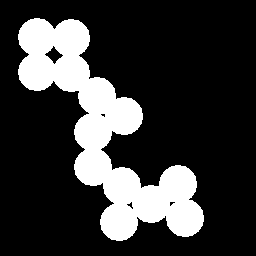
\includegraphics[scale=0.4]{circles}
\end{figure}
\end{frame}

\begin{frame}{Chan-Vese segmentation}
The Chan-Vese segmentation finds the curve $C$ that is the boundary of the segmentation. The way to find that curve is minimizing the following functional:
$$\text{arg min}_{c_1,\ c_2,\ C }\ \mu \text{Lenght}(C) +\nu\text{Area}(inside(C)) +$$$$ \lambda_1\int_{inside(C)}|f(x)-c_1|^2dx + \lambda_2\int_{outside(C)}|f(x)-c_2|^2dx,$$
where $C$ is the boundary of a closed set and $c1$, $c2$ are the values of $u$ respectively inside and outside of $C$. 
\end{frame}

\begin{frame}{Level set functions}
As it is difficult to manipulate $C$ we will use a function $\phi$ and the $C$ will be the zero crossing of $\varphi$ that is 
$$C = \{x\in \Omega:\varphi(x) = 0\}.$$
With this the functional is rewritten as:

$$\text{arg min}_{c_1, c_2, \varphi}\ \mu \int_{\Omega}\delta(\varphi(x))|\nabla\varphi(x)|dx+\nu \int_{\Omega}H(\varphi(x))dx +$$$$ \lambda_1\int_{\Omega}|f(x)-c_1|^2H(\varphi(x))dx + \lambda_2\int_{\Omega}|f(x) -c_2|^2(1-H(\varphi(x)))dx,$$
\end{frame}
\begin{frame}{Level set functions}
In the previous formula $H$ denotes the Heaviside function and $\delta$ the Dirac mass, its distributional derivative:
$$ H = \left\lbrace\begin{array}{l l}
1&t\geq 0,\\
0 & t<0
\end{array}\right. ,\quad \delta(t) = \frac{d}{dt}H(t).$$

Note that we cannot derive $H(t)$. Because of that, in the implementation we take the Heaviside function as
$$H_{\epsilon}(t) = \frac{1}{2}\bigg(1 + \frac{2}{\pi}\arctan \bigg(\frac{t}{\epsilon}\bigg)\bigg)$$
and the Dirac mass as
$$\delta_{\epsilon} = \frac{\epsilon}{\pi(\epsilon^2)+t^2)}$$
\end{frame}



\begin{frame}{Implementation}
Now we have to minimize the functional respect to $c_1$, $c_2$ and $\varphi$.

The way to do it is the following: at each iteration we do this steps:
\begin{enumerate}
\item[1.] Update $c_1$ and $c_2$ as $$c_1 = \frac{\int_{\Omega}f(x)H(\varphi(x))dx}{\int_{\Omega}H(\varphi(x))dx} \text{ and } c_2 = \frac{\int_{\Omega}f(x)(1-H(\varphi(x)))dx}{\int_{\Omega}(1-H(\varphi(x)))dx}$$.
\item [2.] Evolve $\varphi$ using the semi-implicit gradient descent 
$$\varphi_{i,j}^n = [\varphi_{i,j}^n + dt\cdot\delta_{\varepsilon}(\varphi_{i,j}^n)(A_{i,j}\varphi_{i+1,j}^n) + A_{i-1,j}\varphi_{i-1,j}^{n+1}+B_{i,j}\varphi_{i,j+1}^n+$$
$$B_{i, j-1}\varphi_{i,j-1}^{n+1}-\nu - \lambda_1(f_{i,j}-c_1)^2+\lambda_2(_{i,j}-c_2)^2) ]/[1 + dt\cdot\delta_{\varepsilon}(\varphi_{i,j}^n)(A_{i,j} +$$$$ A_{i-1,j} + B_{i,j} + B_{i,j-1})]$$. 
\end{enumerate}
\end{frame}

\begin{frame}{Implementation}

In the previous formula,
$$A_{i,j} = \frac{\mu}{\sqrt{\eta^2 + (\varphi_{i+1,j}^n-\varphi_{i,j}^n)^2+((\varphi_{i,j+1}^n-\varphi_{i,j-1}^{n+1})/2)^2}}$$
$$B_{i,j} = \frac{\mu}{\sqrt{\eta^2+((\varphi_{i+1,j}^n-\varphi_{i-1,j}^{n+1})/2)^2 + (\varphi_{i,j}^n-\varphi_{i+1,j}^n)^2}}$$
\begin{itemize}
\item [3.] If we have reached the maximum number of iterations or the difference $\max(|\varphi^{n+1}-\varphi|)$ is lower than a given tolerance, we stop the algorithm.
\end{itemize}
\end{frame}

\begin{frame}{Results}
Given image of a set of circles. It can be seen that the segmentation takes all the circles as one set.


\begin{figure}
    \centering
    \begin{subfigure}[b]{0.36\textwidth}
        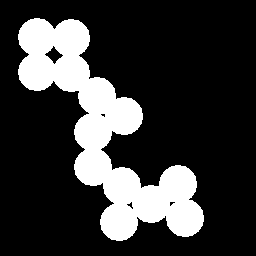
\includegraphics[width=\textwidth]{circles}

    \end{subfigure}
    ~ 
        \begin{subfigure}[b]{0.4\textwidth}
        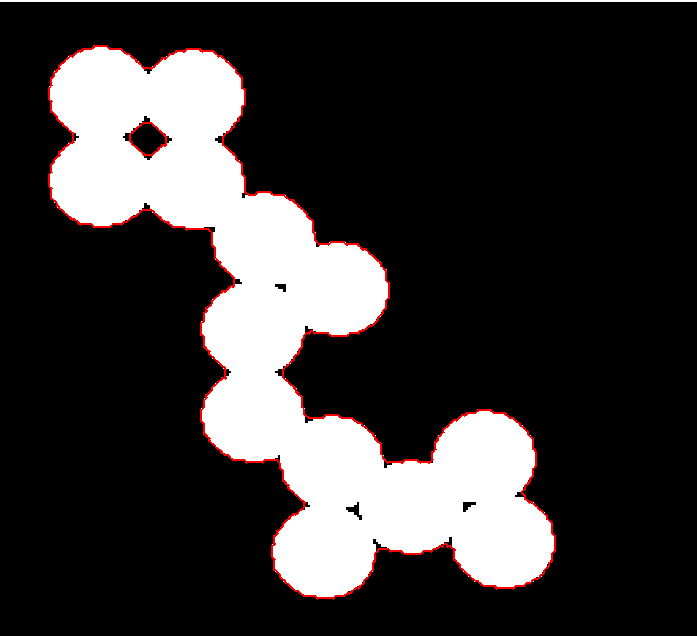
\includegraphics[width=\textwidth]{circles_segmented}

    \end{subfigure}

\end{figure}
\href{run:videos/circles.avi}{\color{red}{Video of the segmentation\footnote{This link and the following that are equal open the video of the segmentation.}}}
\end{frame}

\begin{frame}{Results}
Own image with different objects.  It can be seen that the algorithm can split all the figures.

\begin{figure}
    \centering
    \begin{subfigure}[b]{0.45\textwidth}
        
\includegraphics[width=\textwidth]{Tres_formas}

    \end{subfigure}
    ~ 
        \begin{subfigure}[b]{0.45\textwidth}
        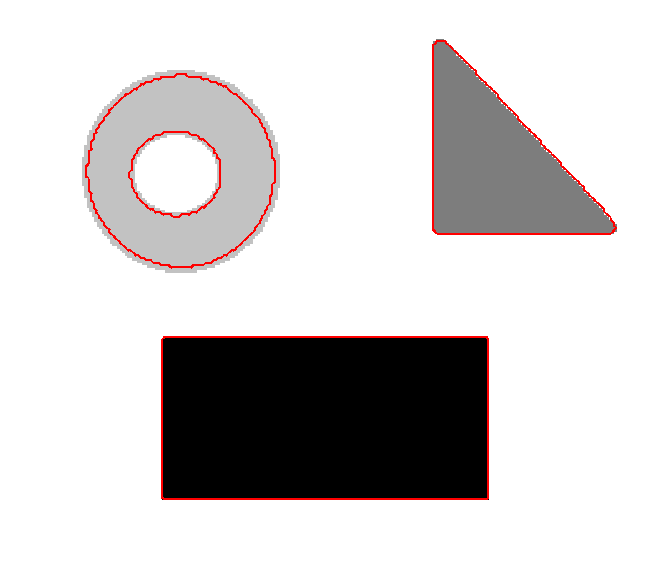
\includegraphics[width=\textwidth]{Tres_formas_segmented}

    \end{subfigure}

\end{figure}
\href{run:videos/Tres_formas.avi}{\color{red}{Video of the segmentation}}
\end{frame}

\begin{frame}{Results}
Segmentation of our goal image, only in the part that do not contain letters. The algorithm makes an smooth segmentation of the part of the image that in the following weeks we would like to inpaint.
\begin{figure}
    \centering
    \begin{subfigure}[b]{0.5\textwidth}
        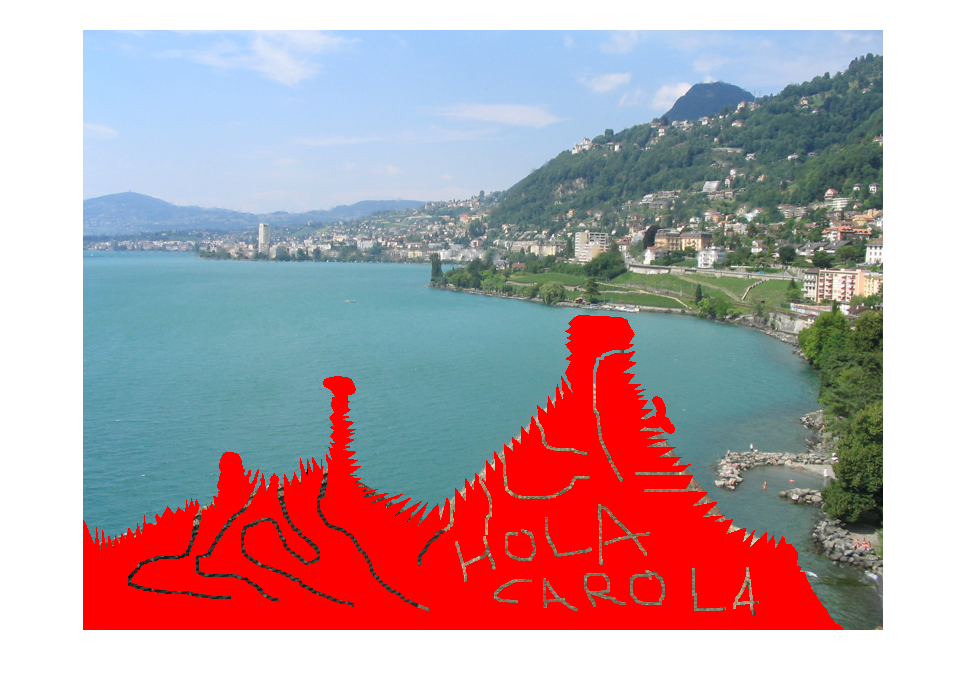
\includegraphics[width=\textwidth]{Goal_Image_inpainted}

    \end{subfigure}
    ~ 
        \begin{subfigure}[b]{0.4\textwidth}
        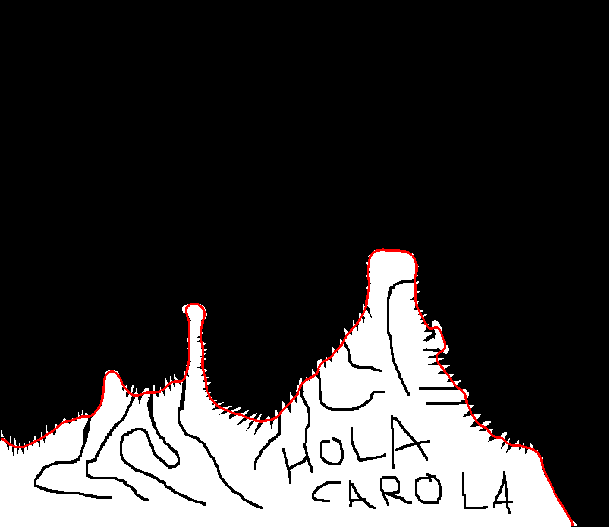
\includegraphics[width=\textwidth]{Goal_Image_segmented}

    \end{subfigure}

\end{figure}

\href{run:videos/Goal_Image.avi}{\color{red}{Video of the segmentation}}
\end{frame}

\begin{frame}{Conclusions}
\begin{itemize}
\item The segmentation of the images is quite good.
\item We don't know under which assumptions the algorithm does not do a correct segmentation.
\item Although its a good algorithm it takes too many iterations to converge.
\end{itemize}
\end{frame}
\end{document}